\documentclass{article}
\usepackage[utf8]{inputenc}
\usepackage{amsthm}
\usepackage{booktabs}
\usepackage{graphicx}
\usepackage{float}
\graphicspath{ {images/} }
\usepackage[margin=1in]{geometry}
\usepackage{tikz}
\usetikzlibrary{arrows,automata,positioning}

\newtheorem*{theorem}{Theorem}

\title{Ata da Reunião}
\date{7 de Outubro de 2016}
\author{Bernardo Meurer\\
        \texttt{86242}
        \and
        Maria Adelaide Ambrósio\\
        \texttt{87064}
        \and
        Inês Coelho\\
        \texttt{87022}}
\begin{document}
\maketitle
\newpage

\begin{center}
\textbf{Contruindo um robot Seguidor de Linha}
\end{center}
\begin{table}[h]
\centering
\begin{tabular}{@{}ll@{}}
Data e Hora & Sexta,  07 de Outubro de 2016 às 09:15h \\ \toprule
Local       & Laboratório Pedro Nunes                \\ \midrule
Presidente  & Rui Vasconcelos                        \\ \midrule
Secretária  & Sofia Varela                            \\ \bottomrule
\end{tabular}
\end{table}
\subsection*{Objetivos}
Debate sobre o planeamento da construção de um robot que segue uma fita preta e
que para quando encontra um obstáculo, retomando a sua marcha quando é avisado.

\subsection*{Tabela MSProject}
\begin{figure}[H]
    \centering
    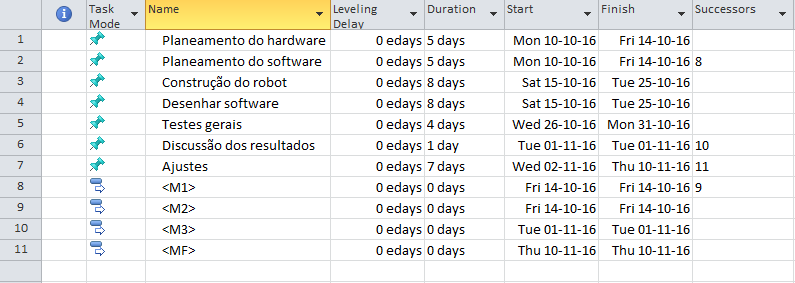
\includegraphics[scale=.8]{geral}
    \caption{Tabela definição do planeamento do projeto}
\end{figure}

\subsection*{Etapas do Projeto}
\begin{enumerate}
    \item Planeamento do Hardware
    \begin{itemize}
        \item Definição da plataforma de desenvolvimento a ser utilizada
              (NXT, Arduino, \dots). Aĺém disso, é necessário desenhar a
              estrutura do robot e selecionar os sensores e motores necessários.
    \end{itemize}
    \item Planeamento do Software
    \begin{itemize}
        \item Temos de definir a lógica a ser usada para que o robot não se
              desvie da linha. Há também que definir a linguagem que deverá ser
              usada e qual o estilo de código e VCS.
    \end{itemize}
    \item Construção do robot
    \begin{itemize}
        \item Testes individuais de cada um dos componentes do robot e
              verificação do funcionamento das partes. Garantir a qualidade e
              durabilidade dos materiais.
    \end{itemize}
    \item Desenvolver o Software
    \begin{itemize}
        \item Implementação do Software como previamente especificado, seguindo
              de forma estrita os padroẽs de código. Adaptar o plano original a
              quaisquer problemas que tenham surgido na etapa 3.
    \end{itemize}
    \item Testes
    \begin{itemize}
        \item Tentar prever todos os tipos de situações de uso do robot e
              submetê-lo a tais condições. Tomar notas rigorosas de falhas e
              possibilidades de melhoria.
    \end{itemize}
    \item Avaliação dos resultados
    \begin{itemize}
        \item Reunir a equipa de desenvolvimento e analisar os resultados dos
              testes feitos na etapa anterior. Definir as melhorias a serem
              realizadas.
    \end{itemize}
    \item Ajustes
    \begin{itemize}
        \item Realizar as melhorias definidas na etapa 6, fazendo adaptações na
              medida do necessário.
    \end{itemize}
\end{enumerate}
\subsection*{PERT}

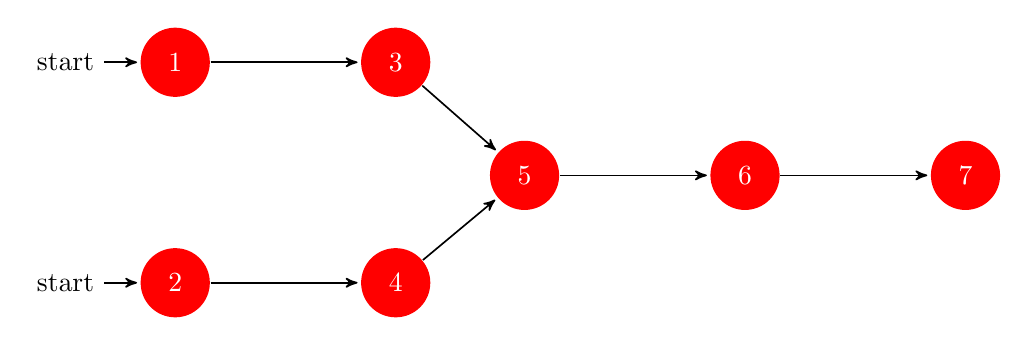
\begin{tikzpicture}[->,>=stealth',shorten >=1pt,auto,node distance=2.8cm,
                    semithick]
  \tikzstyle{every state}=[fill=red,draw=none,text=white]

  \node[state, initial] (A)                         {$1$};
  \node[state, initial] (B) [below of=A]            {$2$};
  \node[state] (C) [right of=A]                     {$3$};
  \node[state] (D) [right of=B]                     {$4$};
  \node[state] (E) [below right=.8cm and 1cm of C]  {$5$};
  \node[state] (F) [right of=E]                     {$6$};
  \node[state] (G) [right of=F]                     {$7$};
  \path (A) edge  node {} (C)
        (B) edge  node {} (D)
        (C) edge  node {} (E)
        (D) edge  node {} (E)
        (E) edge  node {} (F)
        (F) edge  node {} (G);
\end{tikzpicture}
\subsection*{Carta de GANTT}
\begin{figure}[H]
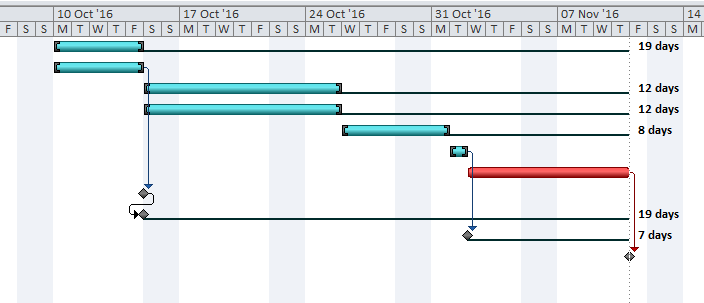
\includegraphics[scale=.8]{gantt}
\caption{Carta de GANTT com a definição das Milestones e da dependência entre
         tarefas para o projeto da contrução do robot}
\end{figure}
\end{document}
